\section{Introduction to tools}
These are the tools that help us to reduce the work of the developer by just providing the function ready for the direct usage. 
\subsection{NetworkX}

\begin{figure}[h]
\centering 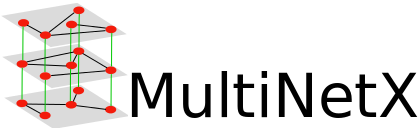
\includegraphics[scale=0.5]{input/images/networkx.png}
\caption{NetworkX logo}
\end{figure}

NetworkX is a Python package for the creation, manipulation, and study of the structure, dynamics, and functions of complex networks.\\

  
{\bf Features}
\begin{itemize}
    \item Data structures for graphs, digraphs, and multigraphs
    \item Many standard graph algorithms
    \item Network structure and analysis measures
    \item Generators for classic graphs, random graphs, and synthetic networks
    \item Nodes can be "anything" (e.g., text, images, XML records)
    \item Edges can hold arbitrary data (e.g., weights, time-series)
    \item Open source 3-clause BSD license
    \item Well tested with over 90\% code coverage
    \item Additional benefits from Python include fast prototyping, easy to teach, and multi-platform
\end{itemize}

{\bf Installation}
\begin{verbatim}
$ sudo apt-get install python-pip python-virtualenv
$ virtualenv venv
$ source venv/bin/activate
$ pip install networkx
\end{verbatim}

{\bf Algorithm}
PageRank computes a ranking of the nodes in the graph G based on the structure of the incoming links. It was originally designed as an algorithm to rank web pages.\\


{\bf Graph types}
\begin{itemize}
\item Undirected Simple
\item Directed Simple
\item With Self-loops
\item With Parallel edges

\end{itemize}

\subsection{OSMnx}

\begin{figure}[h]
\centering 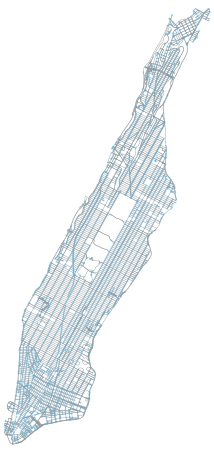
\includegraphics[scale=0.50]{input/images/osmnx.png}
\caption{OSMnx map of manhattan}
\end{figure}
OSMnx: retrieve, construct, analyze, and visualize street networks from OpenStreetMap. OSMnx is a Python package that lets you download spatial geometries and construct, project, visualize, and analyze street networks from OpenStreetMap’s APIs. Users can download and construct walkable, drivable, or bikable urban networks with a single line of Python code, and then easily analyze and visualize them.\\

{\bf Features}
\begin{itemize}
\item Download street networks anywhere in the world with a single line of code
\item Download other infrastructure network types, place polygons, or building footprints as well
\item Download by city name, polygon, bounding box, or point/address + network distance
\item Get drivable, walkable, bikable, or all street networks
\item Visualize the street network as a static image or leaflet web map
\item Simplify and correct the network’s topology to clean and consolidate intersections
\item Save networks to disk as shapefiles or GraphML
\item Conduct topological and spatial analyses to automatically calculate dozens of indicators
\item Calculate and plot shortest-path routes as a static image or leaflet web map
\item Plot figure-ground diagrams of street networks and/or building footprints
\item Download node elevations and calculate edge grades
\item Visualize travel distance and travel time with isoline and isochrone maps
\item Calculate and visualize street bearings and orientations\\

\end{itemize}


{\bf Installation}
\begin{verbatim}
$ sudo apt-get install python-pip python-virtualenv
$ virtualenv venv
$ source venv/bin/activate
$ pip install osmnx
\end{verbatim}

{\bf Usage}
\begin{verbatim}
import osmnx as ox
G = ox.graph_from_place('Punjab, India', network_type='drive')
ox.plot_graph(ox.project_graph(G))
\end{verbatim}